\section{Introduction}

Le système doit actuellement être utilisé par deux applications distinctes pour être fonctionnel à 100\%. De ce fait, cela rends son utilisation moin ergonomique. De plus, de nombreuses fonctionnalités ont été implémentées par Thorlabs, aussi bien dans les logiciels Kinesis que ThorCam qui ne sont pas forcément utilisés dans les manipulations. Cela alourdit leur compréhension. Pour une manipulation de laboratoire, il est donc nécessaire d'avoir une notice suffisamment détaillée pour bien comprendre le fonctionnement du système, installer les logiciels et les configurer. Ce premier point va mener au premier objectif de cette nouvelle application.

Dans l'application Kinesis, il est possible de créer des séquences, c'est à dire d'enregistrer des mouvements sur les servomoteurs X et Y, puis d'allumer le laser, etc... Il est possible de faire une multitude de combinaisons. Cependant, aucun système de vision n'est intégrée et de ce fait, cela rends ces séquences semi-automatiques, demandant une intervention humaine pour des vérifications ou ajustements. Ce second point va mener au deuxième objectif.

\section{Objectifs}
\begin{itemize}[label=\textbullet]
    \item Création de l'application ServoVision qui regroupent les fonctionnalités de base de Kinesis et de ThorCam afin d'avoir qu'une seule application simple d'utilisation. Le nom ServoVision vient de la combinaison de "Servo" pour la gestion des servomoteurs, et "Vision" pour le contrôle de la caméra.
    \item Création d'un algorithme visant à pouvoir détecter automatiquement des particules, ainsi que les déplacer de façon autonome.
\end{itemize}

\newpage
\section{Développement avec Thorlabs}
Thorlabs met à disposition plusieurs outils pour développer sa propre application. Le logiciel Kinesis propose des contrôles .NET utilisables avec des langages comme C\#, Visual Basic, LabVIEW, ou tout autre langage compatible .NET. Des bibliothèques DLL bas niveau sont aussi disponibles.

Du côté de ThorCam, un SDK est fourni pour développer notre propre interface. Un SDK est un kit fourni par Thorlabs qui contient tout le nécessaire (bibliothèques, exemples, docs) pour créer sa propre application.

Grâce à ces bibliothèques et outils, il est donc possible de regrouper les fonctions essentielles de Kinesis et ThorCam dans une seule application personnalisée.

\subsection{Fonctionnalités reprogrammées de Kinesis et ThorCam}

% L'application ServoVision reprend les fonctions utiles pour la manipulation, plus celles ajoutées pour l'algorithme de détection et le déplacement automatique des billes.

Depuis Kinesis, il est possible d'intégrer les blocs en entier que l'on retrouve dans Kinesis pour la gestion des servomoteurs ainsi que du driver du laser (Figure~\ref{laser_driver}), ce qui facilite grandement l'intégration de cette partie dans la nouvelle application.

\begin{figure}[H]
    \begin{center}
        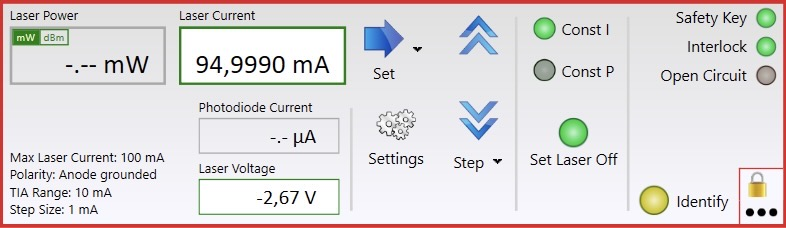
\includegraphics[width=0.65\textwidth]{assets/figures/Application_ServoVision/Laserdriver.jpeg}
    \end{center}
    \captionof{figure}{Bloc qui permet de contrôler le driver du laser en entier}
    \label{laser_driver}
\end{figure}

Depuis ThorCam je programme :
\begin{itemize}[label=\textbullet]
    \item Affichage en direct de la caméra
    \item Pause/Play de la caméra
    \item Capture d'image
    \item Enregistrement d'une vidéo de la caméra
    \item Outils pour mesurer des objets dans l'image
    \item Zoom dans la fenêtre de la caméra
    \item Déplacement dans la fenêtre de la caméra
\end{itemize}

Le but, c'est d'avoir une interface simple, sans toutes les options en plus des logiciels d'origine.

\section{Intégration des fonctionnalités}
\subsection{Contrôle des drivers : laser et servomoteurs}
\subsection{}